\documentclass{llncs}

% \usepackage{showframe}

\usepackage{amssymb}
\usepackage[fleqn]{amsmath}
\usepackage{url}
\usepackage{graphicx}
\usepackage{float}
\usepackage{listings}
\usepackage[ruled,vlined]{algorithm2e}
\usepackage{mathtools}
\usepackage[rightcaption]{sidecap}
\usepackage{multicol}
\usepackage{colortbl}
\usepackage{booktabs}
\usepackage{framed}
%\usepackage{coffee2}
\usepackage{tikz}

\usepackage{color}
\newcommand{\todo}[1]{\textcolor{blue}{#1}}

\usetikzlibrary{shapes, shapes.multipart, arrows, positioning}

\newcommand{\match}{\mathit{match}}
\newcommand{\timeSlot}{\mathit{timeSlot}}
\newcommand{\state}{\mathit{state}}
\newcommand{\change}{\mathit{change}}
\newcommand{\totalChanges}{\mathit{totalChanges}}
\newcommand{\totalBoatChanges}{\mathit{totalBoatChanges}}
\newcommand{\modMatch}{\mathit{modMatch}}
\newcommand{\position}{\mathit{position}}
\newcommand{\imbalance}{\mathit{imbalance}}
\newcommand{\maxImbalance}{\mathit{maxImbalance}}
\newcommand{\timeVar}{\mathit{time}}

\newcommand{\START}{\textnormal{\textsc{Start}}}
\newcommand{\FIRST}{\textnormal{\textsc{First}}}
\newcommand{\MID}{\textnormal{\textsc{Mid}}}
\newcommand{\LAST}{\textnormal{\textsc{Last}}}
\newcommand{\END}{\textnormal{\textsc{End}}}
\newcommand{\BYE}{\textnormal{\textsc{Bye}}}

\newcommand{\eachOccursExactlyOnce}{\mathrm{eachOccursExactlyOnce}}
\newcommand{\allDifferent}{\mathrm{allDifferent}}
\newcommand{\validStateSequence}{\mathrm{validStateSequence}}
\newcommand{\minimise}{\mathrm{minimise}}
\newcommand{\maximum}{\mathrm{maximum}}

\DeclarePairedDelimiter\abs{\lvert}{\rvert}

\newcommand\nldots{\,\hbox to 0.8em{.\hss.\hss.}\,}

\sidecaptionvpos{table}{c}

\definecolor{uofgheather}{rgb}{0.356863, 0.32549, 0.490196}
\definecolor{uofgaquamarine}{rgb}{0.603922, 0.72549, 0.678431}
\definecolor{uofgslate}{rgb}{0.309804, 0.34902, 0.380392}
\definecolor{uofgrose}{rgb}{0.823529, 0.470588, 0.709804}
\definecolor{uofgmocha}{rgb}{0.709804, 0.564706, 0.47451}

\definecolor{uofglawn}{rgb}{0.517647, 0.741176, 0}
\definecolor{uofgcobalt}{rgb}{0, 0.615686, 0.92549}
\definecolor{uofgturquoise}{rgb}{0, 0.709804, 0.819608}
\definecolor{uofgsunshine}{rgb}{1.0, 0.862745, 0.211765}
\definecolor{uofgpumpkin}{rgb}{1.0, 0.72549, 0.282353}
\definecolor{uofgthistle}{rgb}{0.584314, 0.070588, 0.447059}
\definecolor{uofgpillarbox}{rgb}{0.701961, 0.047059, 0}
\definecolor{uofglavendar}{rgb}{0.356863, 0.301961, 0.580392}

\begin{document}

\title{Constructing Sailing Match Race Schedules: Round Robin Pairing Lists}
\titlerunning{Match Race Scheduling}
%\toctitle{}
\author{Craig Macdonald \and Ciaran McCreesh \and Alice Miller \and Patrick Prosser}
\institute{University of Glasgow, Glasgow, Scotland \\ \email{patrick.prosser@glasgow.ac.uk}}
\authorrunning{Macdonald, McCreesh, Miller, Prosser}
\maketitle

\begin{abstract} 
\todo{We encourage industrial and academic users of constraint technology to submit papers on completed or on-going practical projects. Papers comparing constraint technology to other optimization techniques (MIP, local search, SAT, etc.) on a realistic application with a sound experimental evaluation are also encouraged. Papers which clearly define users' benefits, describe the required effort to build the application and the time frame in which it was delivered, will match the acceptance criteria most closely. The novelty of the application domain, while potentially a plus, is not the only deciding acceptance criterion. Application papers will be reviewed by a program committee with significant experience in the use of CP in applications. The writing of the paper should be guided by providing answers to four main questions: Problem being solved? Why CP? How CP? Added value of CP? Formatting, length, and dates for submissions are the same as for the technical track.}
\end{abstract}

\section{Introduction}
%\coffee{1}
This work describes a round robin competition format that arises from sailing, known as match racing. Competitors, i.e. {\em skippers}, compete against each other in a series of matches taking place in rounds, known as {\em flights}.  A match is composed of two skippers, with each skipper in a boat on his own. Skippers in a match set off together, one on the port side, the other starboard, and first home wins that match. ISAF World Sailing rules dictate what makes a legal schedule and what criteria to optimise. This is a rich set of rules, 13 in all, and as far as we know, all published schedules have been produced by hand. This is a daunting task. A close inspection of these schedules reveals that most are illegal, violating many of the match race rules, many schedules are missing and some that are legal are far from optimal.

This paper describes the scheduling problem. We present a constraint programming solution and document how this model was constructed incrementally. We believe this illustrates how adaptable constraint programming is, i.e. given a fairly robust model this can be incrementally developed to address all of the required criteria. Our schedules are then constructed in a sequence of stages, not dissimilar to the hybrid and decomposition based approaches in \cite{lombardi2012}. Some ISAF published schedules are presented along with some of our own, some of these being new.  These schedules are esentially blank forms, made available to umpires and competition managers. These forms are then filled in with names of actual competitors, i.e. these schedules are reusable.

The paper is organised as follows: we present the 13 match racing rules and then the constraint models and four stages of schedule construction, schedules are then presented, there is then a discuss and we conclude.


\section{Problem Definition: Round Robin Pairing Lists}\label{sec:definition}
The guidelines for running match racing events~\cite{isaf} places a number of criteria on how the competing skippers are scheduled into flights and matches, known as pairing lists. Several of these criteria are applicable when the number of skippers exceeds the number of available boats, in which case skippers have to change in and out of boats, and are allowed time in the schedule to check and fine-tune the boat they change into. Typically, matches set off at 5 minute intervals with each match taking about 20 minutes. Therefore, if we have 10 skippers and 10 boats we have 45 matches. This results in 9 flights each of 5 matches.  Each flight takes about 50 minutes, consequently eight or nine flights a day is a reasonable achievement for most umpires. Consequently, the number of boats and skippers involved is typically small.

The criteria for generated match racing schedules (pairing lists) are given in ISAF ``International Umpires' and Match Racing Manual'' \cite{isaf}, section
M.2 Recommended Criteria for Round Robin Pairing Lists, and are detailed below.

\begin{framed}
\begin{enumerate}
\item Each skipper sails against each other skipper once.
\item *When skippers have an even number of matches, they have the same number of port and starboard assignments.
\item *When skippers have an odd number of matches, the first half of the skippers
    will have one more starboard assignment.
%\item When there is an even number of flights, each skipper has the same number
%    of port and starboard assignments.
%\item When there is an odd number of flights, the first half of the skippers
%    will have one more starboard assignment.
\item No skipper in the last match of a flight should be in the first match of
    the next flight.
\item No skipper should have more than two consecutive port or starboard
    assignments.
\item Each skipper should be assigned to match 1, match 2, etc. in a flight as
    equally as possible.
\item In flights with five or more matches, no skipper should be in the
    next-to-last match in a flight and then in the first match of the next
    flight.
\item If possible, a skipper should be starboard when meeting the nearest
    lowest ranked skipper (i.e.\ \#1 will be starboard against \#2, \#3 will be
    starboard against \#4).
\item Close-ranked skippers meet in the last flight.
\item Minimise the number of boat changes.
\item Skippers in the last match of a flight do not change boats.
\item Skippers in new boats do not sail in the first match of the next flight.
\item Skippers have a reasonable sequence of matches and blanks.
\end{enumerate}
Note that criteria 10, 11 and 12 only apply when there are fewer boats than
skippers.
\end{framed}

We have rephrased criteria 2 \& 3 (denoted *) to clarify an error in \cite{isaf}. Note that the order of matches within a flight is significant and is constrained, as is the order of flights within a schedule and the position of skippers within a match. This permits fair schedules that provide the opportunity for skippers to change boats, take fair advantage of wind direction, etc. 

Criteria 12 defines what is meant by a boat change: if in flight $i$ this skipper is not in a match (i.e. it is a bye for this skipper) but is in a match in flight $i+1$ then he has to get into a boat, rearrange all his kit and set the boat as he likes it prior to casting off, and this is a boat change.

Next, we note that skippers can be ranked prior to an event -- based on their performance in previous events~\footnote{\url{http://www.sailing.org/rankings/match/}} -- which is used to seed the skippers. The ordering of skippers within a match signifies their starting position (port or starboard) -- as skippers allocated the starboard starting position gain a small competitive advantage in that match - criteria 8 accomplishes the seedings.

Criteria 10 is ambiguous: - this could be interpreted on a schedule basis: i.e.\ to minimise the overall number of changes in the entire pairing list schedule; or alternatively as well as a fair, but minimal number of changes across all skippers. In our work, we take the latter viewpoint.

There are some conflicts inherent in the rules. Take criteria 4 and 11, assume we have 4 boats, and in flight $i$ the last match is the pair of skippers ($x,y$). Criteria 11 dictates that skippers $x$ and $y$ must appear in the next flight, $i+1$, and criteria 4 that neither can be first in the next flight. This forces skippers $x$ and $y$ to compete in flight $i+1$ as the last match, violating criteria 1. Therefore, although not explicitly stated, there are no legal schedules with less than 6 boats.

\section{The Constraint Models}\label{sec:models}

The schedules are produced in four stages. The first stage produces a schedule
that respects criteria 1, 4, 11 and 12, and minimises criteria 10 (boat
changes). The second stage constructs a schedule that respects criteria 1, 4,
11, 12 (again), has criteria 10 as a hard constraint generated from first
stage, and minimises criteria 6 (balance). This results in a schedule that
attempts to minimise boat changes \emph{and} balance. The third stage satisfies
criteria 9, and is a simple translation of the schedule produced in stage 2.
The final stage orients skippers within matches to address criteria 2, 3, 5
and 8.

We now describe the constraint models and processes used in each stage. In the
text below we assume there are $n$ skippers and $b$ boats, with $m = b/2$
matches in a flight. In total there are $t = n(n-1)/2$ matches and $f = \lceil
n(n-1)/m  \rceil$ flights. We use the schedule in Table~\ref{tab1}, for 7
skippers and 6 boats, to help illustrate the constraint models. Our
descriptions of the models omit some minor details, however the models are
available to download\footnote{?? give us a link to the models}.

\begin{SCtable}[1.8][tb]
    \setlength{\tabcolsep}{3pt}
    \begin{tabular}{cccc}
        \toprule
        Flight & \multicolumn{3}{c}{Matches} \\ \midrule
        0 & (0,1) & (2,3) & (4,5) \\
        1 & (0,2) & (4,6) & (1,5) \\
        2 & (2,6) & (0,5) & (1,3) \\
        3 & (5,6) & (0,3) & (1,4) \\
        4 & (3,5) & (1,6) & (2,4) \\
        5 & (3,6) & (0,4) & (2,5) \\
        6 & (3,4) & (1,2) & (0,6) \\ \bottomrule
    \end{tabular}
    \caption{A round-robin schedule with 7 skippers, 6 boats and 7 flights.
        Skippers are numbered 0 to 6. Note that the order of skippers within a flight
        is significant, as is position within a match (port or starboard). This
        schedule is the result of stages 1 and 2, and has yet to be renumbered and
        oriented (stages 3 and 4).} \label{tab1}
\end{SCtable}

\subsection{Stage 1: Minimising Boat Changes}

\paragraph{Modeling skippers:} The first thing we model, in the first half of
Figure~\ref{model:stage1}, is a skipper. Each skipper $\sigma$ has a temporal
view of his schedule in the array of constrained integer variables
$\timeSlot[0]$ to $\timeSlot[{t-1}]$, and a state view in the array of
constraint integer variables $\state[0]$ to $\state[{f-1}]$. The state of this
skipper in flight $i$ is found in $\state[i]$, and this corresponds to
timeslots $\timeSlot[{i \cdot m}]$ to $\timeSlot[{m(i+1)-1}]$.

\begin{figure}[p]
\setlength{\mathindent}{1em}
\setlength{\abovedisplayskip}{0pt}
\setlength{\belowdisplayskip}{0pt}
\setlength{\abovecaptionskip}{0pt}
\begin{framed}
\begin{align}
    \intertext{A copy of these variables and constraints is created for each skipper $\sigma$:\smallskip}
    &\forall \tau \in \{0 \nldots t{-}1\}: \timeSlot[{\tau}] \in \{{-}2 \nldots t{-}1\} \setminus \{\sigma\} \label{var:timeSlot} \tag{V1} \\
    &\forall i \in \{0 \nldots f{-}1\}: \state[{i}] \in \{\FIRST,\MID,\LAST,\BYE,\END\} \label{var:state} \tag{V2} \\
    &\forall i \in \{0 \nldots f\}: \label{C1} \tag{C1} \\
    &\begin{alignedat}{3}
    &\hspace*{1em} \state[{i}] = \FIRST &\ &\Leftrightarrow&&\ \timeSlot[{m \cdot i}] \geq 0 \\
    &\hspace*{1em} \state[{i}] = \MID   &\ &\Leftrightarrow&&\ \exists j \in \{m \cdot i + 1 \nldots m \cdot (i + 1) - 2\} : \timeSlot[{j}] \geq 0 \\
    &\hspace*{1em} \state[{i}] = \LAST  &\ &\Leftrightarrow&&\ \timeSlot[m \cdot (i + 1) - 1] \geq 0 \\
    &\hspace*{1em} \state[{i}] = \BYE   &\ &\Leftrightarrow&&\ \forall j \in \{m \cdot i \nldots m \cdot (i + 1) - 1\} : \timeSlot[j] = -1 \\
    &\hspace*{1em} \state[{i}] = \END   &\ &\Leftrightarrow&&\ \forall j \in \{m \cdot i \nldots m \cdot (i + 1) - 1\} : \timeSlot[j] = -2
    \end{alignedat} \nonumber \\
    &\eachOccursExactlyOnce(\timeSlot, \{0, \nldots, n{-}1\} \setminus \{\sigma\}) \label{C2} \tag{C2} \\
    &\validStateSequence(\state) \label{C3} \tag{C3} \\[0.1cm]
    & \forall i \in \{0 \nldots f{-}2\}: \change[{i}] \in \{0,1\} \label{V3} \tag{V3} \\
    & \totalChanges \in \mathbb{N} \label{V4} \tag{V4} \\
    & \forall i \in \{0 \nldots f{-}2\}: \change[{i}] = 1 \Leftrightarrow \state[{i}] = \BYE \wedge \state[{i + 1}] \neq \BYE \label {C4} \tag{C4} \\
    & \totalChanges = \textstyle\sum \change \label{C5} \tag{C5}
\end{align}
\end{framed}\begin{framed}
\begin{align}
    \intertext{Match and temporal perspectives:\smallskip}
    & \forall i \in \{0 \nldots n{-}2\} : \forall j \in \{ i{+}1 \nldots n{-}1 \} : \nonumber \\
    & \hspace*{1em} \match[{i,j}] \in \{0..t{-}1\} \tag{V5} \label{V5} \\
    & \hspace*{1em} \match[{j,i}] \equiv \match[{i,j}] \nonumber \\
    & \hspace*{1em} \forall k \in \{0 \nldots t{-}1 \} : \nonumber \\
    & \hspace*{2em} \match[{i,j}] = k \Leftrightarrow \sigma[{i}].\timeSlot[{k}] = j \wedge \sigma[{j}].\timeSlot[{k}] = i \tag{C6} \label{C6} \\[0.1cm]
    & \forall i \in \{0 \nldots n{-}2\} : \forall j \in \{ i{+}1 \nldots n{-}1 \} \nonumber : \\
    & \hspace*{1em} \modMatch[{i,j}] \in \{0..f{-}1\} \label{V6} \tag{V6} \\
    & \hspace*{1em} \modMatch[{j,i}] \equiv \modMatch[{i,j}] \nonumber  \\
    & \hspace*{1em} \modMatch[{i,j}] = \match[{i,j}] / m \tag{C7} \label{C7} \\
    & \forall i \in \{0 \nldots n{-}1 \} : \allDifferent(\modMatch[{i}]) \tag{C8} \label{C8} \\[0.1cm]
    & \forall \tau \in \{0 \nldots t{-}1 \} : \nonumber \\
    & \hspace*{1em} \timeVar[{\tau}] \in \{(0,1) \nldots (n{-}2,n{-}1)\} \tag{V7} \label{V7} \\
    & \hspace*{1em} \forall i \in \{0 \nldots n{-}2\} : \forall  j \in \{ i{+}1 \nldots n{-}1 \} : \timeVar[{\tau}] = (i,j) \Leftrightarrow \match[{i,j}] = \tau \tag{C9} \label{C9} \\[0.1cm]
    & \totalBoatChanges = \textstyle\sum \sigma.\totalChanges \label{V8} \tag{V8} \\
    & \minimise(\totalBoatChanges) \label{C10} \tag{C10}
\end{align}
\end{framed}
\caption{Our constraint model, from a skipper perspective (top) and a match and
temporal perspective (below). The number of skippers is $n$, and $m$ is the
number of matches in a flight. The number of flights is $f = \lceil n(n-1)/m
\rceil$, and there are $t = n(n-1)/2$ matches in total.}\label{model:stage1}
\end{figure}

In \eqref{var:timeSlot} the array $\timeSlot$ is defined and in
\eqref{var:state}, $\state$ is defined. If variable $\timeSlot[{i}] = k$ and $k
\geq 0$ then this skipper is in a match with skipper~$k$ at time~$i$. Variable
$\state[{i}]$ gives the state of this skipper in flight~$i$. The cases in
\eqref{C1} say that a skipper can be in a match in the first time slot in the
flight, or in the middle of the flight\footnote{\ldots actually, not first and
not last.}, or in the last time slot of the flight. Alternatively, if all time
slots in a flight are equal to $-1$ then the skipper is in a bye, and if all time
slots in a flight are equal to $-2$ then the skipper has finished all his
matches.

We must then ensure that each skipper $\sigma$ is in a match with all other
skippers $\{0, \nldots, n-1\} \setminus \{\sigma\}$. This is \eqref{C2}, which
may be implemented by imposing a global cardinality constraint \cite{globCard}
on the array $\timeSlot$.

\paragraph{State transitions:} The $\state$ variables are then used to impose
match race criteria 4 (if last in flight $i$ then not first in flight $i+1$),
criteria 11 (if last in flight $i$ then not in a bye in flight $i+1$) and
criteria 12 (if flight $i$ is a bye then flight $i$ is not first).  These
criteria are imposed by \eqref{C3}, which is a deterministic finite automata
(DFA) constraint \cite{Pesant04}. The transitions for the DFA are shown
pictorially in Figure~\ref{skipper5}: arcs represent a transition from one
state to another. The DFA is encoded as a set of transition objects $\langle
q_{i},\iota,q_{j} \rangle$, where a transition is made from state $q_{i}$ to
state $q_{j}$ when encountering input $\iota$. In addition we specify the
accepting states, which are all states except the start state (white) and the
bye state (pink).  This constraint also ensures that if a skipper has finished
his matches in flight $i$ (i.e.\ $\END$) then he has finished his matches in
flight $i+1$ (and so on).

Figure~\ref{skipper5} also shows the skipper-oriented variables and constraints
corresponding to skipper 5 in the Table~\ref{tab1} schedule. The $\state$ array
is presented as coloured boxes, and below that is the $\timeSlot$ array. The
arrows represent the channeling constraints \eqref{C1}. The
$\state$ array is coloured with green representing $\LAST$, yellow for $\MID$, blue
for $\FIRST$, red for $\LAST$ and (not shown) pink for $\BYE$. The schedule of
Table~\ref{tab1} is reproduced with the matches for skipper 5 emboldened.

\paragraph{Boat changes:} A boat change occurs when a skipper has been in a
$\BYE$ state in flight $i$ and then is in a match in the next flight $i+1$.
This is encoded using the array of zero/one variables \eqref{V3}, and the
constraint \eqref{C4}, and accumulated into $\totalChanges$
(\ref{V4},~\ref{C5}).

\begin{figure}[tb]
    \centering
    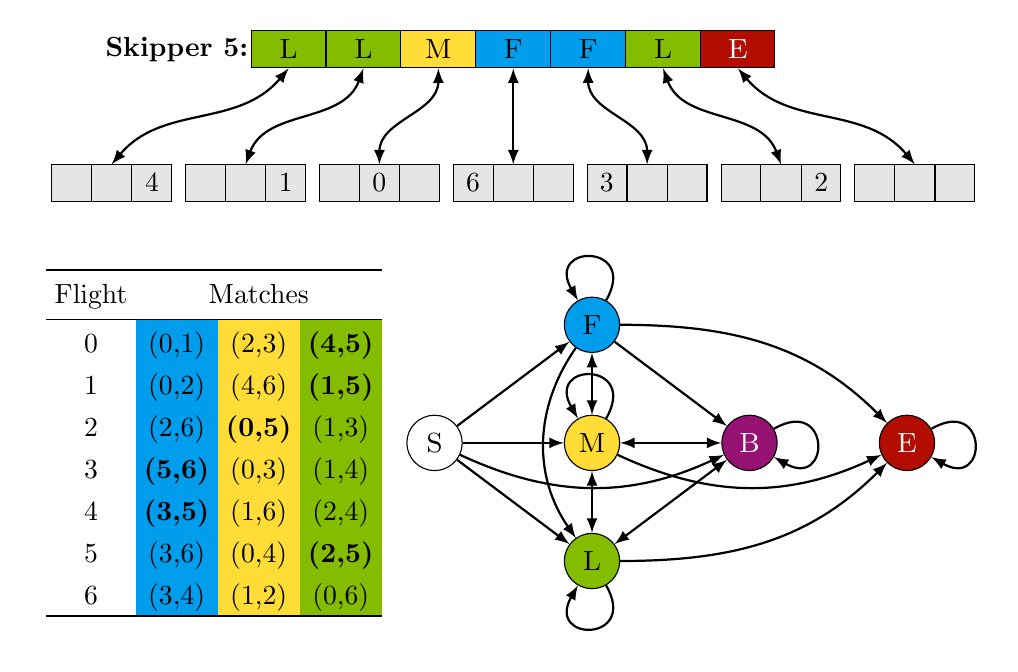
\begin{tikzpicture}
    \begin{scope}[every node/.style={minimum size=2em,inner sep=1}, xshift=-1cm]
        \node (DFAS) [draw, circle, fill=white]                     at (0,  0)   { \textsc{S} };
        \node (DFAF) [draw, circle, fill=uofgcobalt]                at (2,  1.5) { \textsc{F} };
        \node (DFAM) [draw, circle, fill=uofgsunshine]              at (2,  0)   { \textsc{M} };
        \node (DFAL) [draw, circle, fill=uofglawn]                  at (2, -1.5) { \textsc{L} };
        \node (DFAB) [draw, circle, fill=uofgthistle, text=white]   at (4,  0)   { \textsc{B} };
        \node (DFAE) [draw, circle, fill=uofgpillarbox, text=white] at (6,  0)   { \textsc{E} };

        \draw [->, >=latex, thick] (DFAS) to (DFAF);
        \draw [->, >=latex, thick] (DFAS) to (DFAM);
        \draw [->, >=latex, thick] (DFAS) to (DFAL);
        \draw [->, >=latex, thick] (DFAS) to [out=-25, in=-155] (DFAB);

        \draw [->, >=latex, thick] (DFAF) to [out=60, in=120, looseness=6] (DFAF);
        \draw [->, >=latex, thick] (DFAF) to [out=-125, in=125] (DFAL);
        \draw [->, >=latex, thick] (DFAF) to (DFAB);
        \draw [->, >=latex, thick] (DFAF) to [out=0, in=135] (DFAE);

        \draw [<->, >=latex, thick] (DFAF) to (DFAM);

        \draw [->, >=latex, thick] (DFAM) to [out=60, in=120, looseness=6] (DFAM);
        \draw [->, >=latex, thick] (DFAM) to [out=-25, in=-155] (DFAE);

        \draw [<->, >=latex, thick] (DFAM) to (DFAB);
        \draw [<->, >=latex, thick] (DFAM) to (DFAL);

        \draw [->, >=latex, thick] (DFAL) to [out=300, in=240, looseness=6] (DFAL);
        \draw [->, >=latex, thick] (DFAL) to [out=0, in=225] (DFAE);

        \draw [<->, >=latex, thick] (DFAL) to (DFAB);

        \draw [->, >=latex, thick] (DFAB) to [out=30, in=-30, looseness=6] (DFAB);

        \draw [->, >=latex, thick] (DFAE) to [out=30, in=-30, looseness=6] (DFAE);
    \end{scope}

    \begin{scope}[yshift=5cm, scale=0.85]
        \node at (-5, 0) { \textbf{ Skipper 5: } };

        \node (AllArray) [anchor=center, draw, rectangle split, rectangle split horizontal, rectangle split parts=7,
            rectangle split part fill={uofglawn,uofglawn,uofgsunshine,uofgcobalt,uofgcobalt,uofglawn,uofgpillarbox}] at (0, 0) {
            \nodepart[text width=2em, align=center] {one}   \textsc{L}
            \nodepart[text width=2em, align=center] {two}   \textsc{L}
            \nodepart[text width=2em, align=center] {three} \textsc{M}
            \nodepart[text width=2em, align=center] {four}  \textsc{F}
            \nodepart[text width=2em, align=center] {five}  \textsc{F}
            \nodepart[text width=2em, align=center] {six}   \textsc{L}
            \nodepart[text width=2em, align=center, text=white] {seven} \textsc{E}
        };

        \node (Array1) [anchor=center, draw, rectangle split, rectangle split horizontal, rectangle split parts=3,
            rectangle split part fill={black!10!white,black!10!white,black!10!white}]  at (-6, -2) {
            \nodepart[text width=0.75em, align=center] {one}
            \nodepart[text width=0.75em, align=center] {two}
            \nodepart[text width=0.75em, align=center] {three} 4
        };

        \node (Array2) [anchor=center, draw, rectangle split, rectangle split horizontal, rectangle split parts=3,
            rectangle split part fill={black!10!white,black!10!white,black!10!white}]  at (-4, -2) {
            \nodepart[text width=0.75em, align=center] {one}
            \nodepart[text width=0.75em, align=center] {two}
            \nodepart[text width=0.75em, align=center] {three} 1
        };

        \node (Array3) [anchor=center, draw, rectangle split, rectangle split horizontal, rectangle split parts=3,
            rectangle split part fill={black!10!white,black!10!white,black!10!white}]  at (-2, -2) {
            \nodepart[text width=0.75em, align=center] {one}
            \nodepart[text width=0.75em, align=center] {two} 0
            \nodepart[text width=0.75em, align=center] {three}
        };

        \node (Array4) [anchor=center, draw, rectangle split, rectangle split horizontal, rectangle split parts=3,
            rectangle split part fill={black!10!white,black!10!white,black!10!white}]  at (0, -2) {
            \nodepart[text width=0.75em, align=center] {one} 6
            \nodepart[text width=0.75em, align=center] {two}
            \nodepart[text width=0.75em, align=center] {three}
        };

        \node (Array5) [anchor=center, draw, rectangle split, rectangle split horizontal, rectangle split parts=3,
            rectangle split part fill={black!10!white,black!10!white,black!10!white}]  at (2, -2) {
            \nodepart[text width=0.75em, align=center] {one} 3
            \nodepart[text width=0.75em, align=center] {two}
            \nodepart[text width=0.75em, align=center] {three}
        };

        \node (Array6) [anchor=center, draw, rectangle split, rectangle split horizontal, rectangle split parts=3,
            rectangle split part fill={black!10!white,black!10!white,black!10!white}]  at (4, -2) {
            \nodepart[text width=0.75em, align=center] {one}
            \nodepart[text width=0.75em, align=center] {two}
            \nodepart[text width=0.75em, align=center] {three} 2
        };

        \node (Array7) [anchor=center, draw, rectangle split, rectangle split horizontal, rectangle split parts=3,
            rectangle split part fill={black!10!white,black!10!white,black!10!white}]  at (6, -2) {
            \nodepart[text width=0.75em, align=center] {one} \phantom{1}
            \nodepart[text width=0.75em, align=center] {two}
            \nodepart[text width=0.75em, align=center] {three}
        };

        \draw [<->, thick, >=latex] (AllArray.one south) to [in=50, out=230] (Array1.two north);
        \draw [<->, thick, >=latex] (AllArray.two south) to [in=70, out=250] (Array2.two north);
        \draw [<->, thick, >=latex] (AllArray.three south) to [in=90, out=270] (Array3.two north);
        \draw [<->, thick, >=latex] (AllArray.four south) to [in=90, out=270] (Array4.two north);
        \draw [<->, thick, >=latex] (AllArray.five south) to [in=90, out=270] (Array5.two north);
        \draw [<->, thick, >=latex] (AllArray.six south) to [in=110, out=290] (Array6.two north);
        \draw [<->, thick, >=latex] (AllArray.seven south) to [in=130, out=310] (Array7.two north);
    \end{scope}

    \begin{scope}
        \node at (-3.8, 0) {
            \begin{minipage}{4.5cm}
                \centering
                \setlength{\tabcolsep}{3pt}
                \setlength{\aboverulesep}{0pt}
                \setlength{\belowrulesep}{0pt}
                \setlength{\extrarowheight}{.75ex}
                \begin{tabular}{c>{\columncolor{uofgcobalt}}c>{\columncolor{uofgsunshine}}c>{\columncolor{uofglawn}}c}
                    \toprule
                    Flight & \multicolumn{3}{c}{Matches} \\[2pt] \midrule
                    0 & (0,1) & (2,3) & \textbf{(4,5)} \\
                    1 & (0,2) & (4,6) & \textbf{(1,5)} \\
                    2 & (2,6) & \textbf{(0,5)} & (1,3) \\
                    3 & \textbf{(5,6)} & (0,3) & (1,4) \\
                    4 & \textbf{(3,5)} & (1,6) & (2,4) \\
                    5 & (3,6) & (0,4) & \textbf{(2,5)} \\
                    6 & (3,4) & (1,2) & (0,6) \\ \bottomrule
                \end{tabular}
            \end{minipage}
        };
    \end{scope}

    \end{tikzpicture}
    \caption{A pictorial representation of a skipper (skipper 5) with multicoloured
        state and grey timeslots. The schedule for skipper 5 is in bold and the
        deterministic finite automata for criteria 4, 11 and 12 is drawn with state
        $\START$ in white, $\FIRST$ in blue, $\MID$ in yellow, $\LAST$ in green, $\BYE$
    in pink and $\END$ in red.}\label{skipper5}
\end{figure}

\paragraph{Match perspective:} We are now in a position to model criteria 1
(each skipper sails against every other skipper) and optimisation criteria 10
(minimise boat changes).  In the second half of Figure~\ref{model:stage1} we
present a match perspective of the schedule, using a two dimensional array of
variables $\match$ \eqref{V5}, where $\match[{i,j}]$ is the time slot that
skippers $\sigma[{i}]$ and $\sigma[{j}]$ meet in a match. Only the half above
the diagonal is represented, and the lower half is made up of exactly the same
variables, i.e.\ $\match[{i,j}]$ is \emph{exactly} the same constrained
variable as $\match[{j,i}]$. Constraint \eqref{C6} states that  a match between
skippers $\sigma[{i}]$ and $\sigma[{j}]$ takes place at time $k$ (i.e.\
$\match[{i,j}] = k$) if and only if  skipper $\sigma[{i}]$'s $k^{th}$ time slot
is skipper $\sigma[{j}]$ and conversely that skipper $\sigma[{j}]$'s $k^{th}$
time slot is skipper $\sigma[{i}]$). Variables \eqref{V6} and constraints
\eqref{C7} then convert this from time slots to flights, i.e.\
$\modMatch[{i,j}]$ is the flight in which skippers $\sigma[{i}]$ and
$\sigma[{j}]$ meet for a match. Finally, constraint \eqref{C8} ensures that
each skipper's match occurs in different flights. Also, since $\modMatch[{i,j}]
\equiv \modMatch[{j,i}]$, setting rows to be all different also ensures that
columns are all different.

\paragraph{Temporal perspective:} We now take a temporal view \eqref{V7}, such
that $\timeVar[{\tau}]$ is a pair $(i,j)$, stating that at time $\tau$ skippers
$\sigma[{i}]$ and $\sigma[{j}]$ are in a match. We channel between the match
perspective and the temporal perspective using \eqref{C9}.

\paragraph{Optimisation criteria:} Finally we have the optimisation criteria
(criteria 10) to minimise the number of boat changes. This is handled by
\eqref{V8} and \eqref{C10}.

\paragraph{Decision variables:} The decision variables are $\timeVar[{0}]$ to
$\timeVar[{t-1}]$, i.e.\ for each time slot we decide what match takes place. A
symmetry break is made at the top of search by forcing the first round to
contain the matches $(0,1), (2,3), \nldots$, i.e.\ $\forall i \in \{0 \nldots
{m-1}\} : \match[{2i, 2i+1}] = i$.

\bigskip \noindent
Figure \ref{schedChanges} gives a pictorial view of the entire model, using the
7 skipper and 6 boat problem. On the right we have the 7 skippers with their
states and time slots. Again, top right, we give the schedule actually
produced.  Middle left we have the $\match$ array and at the bottom the
$\timeVar$ array. Above the $match$ array we have the $\modMatch$ array. The
yellow arrows show the channeling between parts of the model.

The schedule presented has 6 boat changes: there are no boat changes in flight
0 (first flight), in flight 1 skipper 6 has a boat change, in flight 2 skipper
3 has a boat change, in flight 3 skipper 4, in flight 4 skipper 6, in flight 5
skipper 0, and flight 6 skipper 1.

\begin{figure}[tb]
\centering
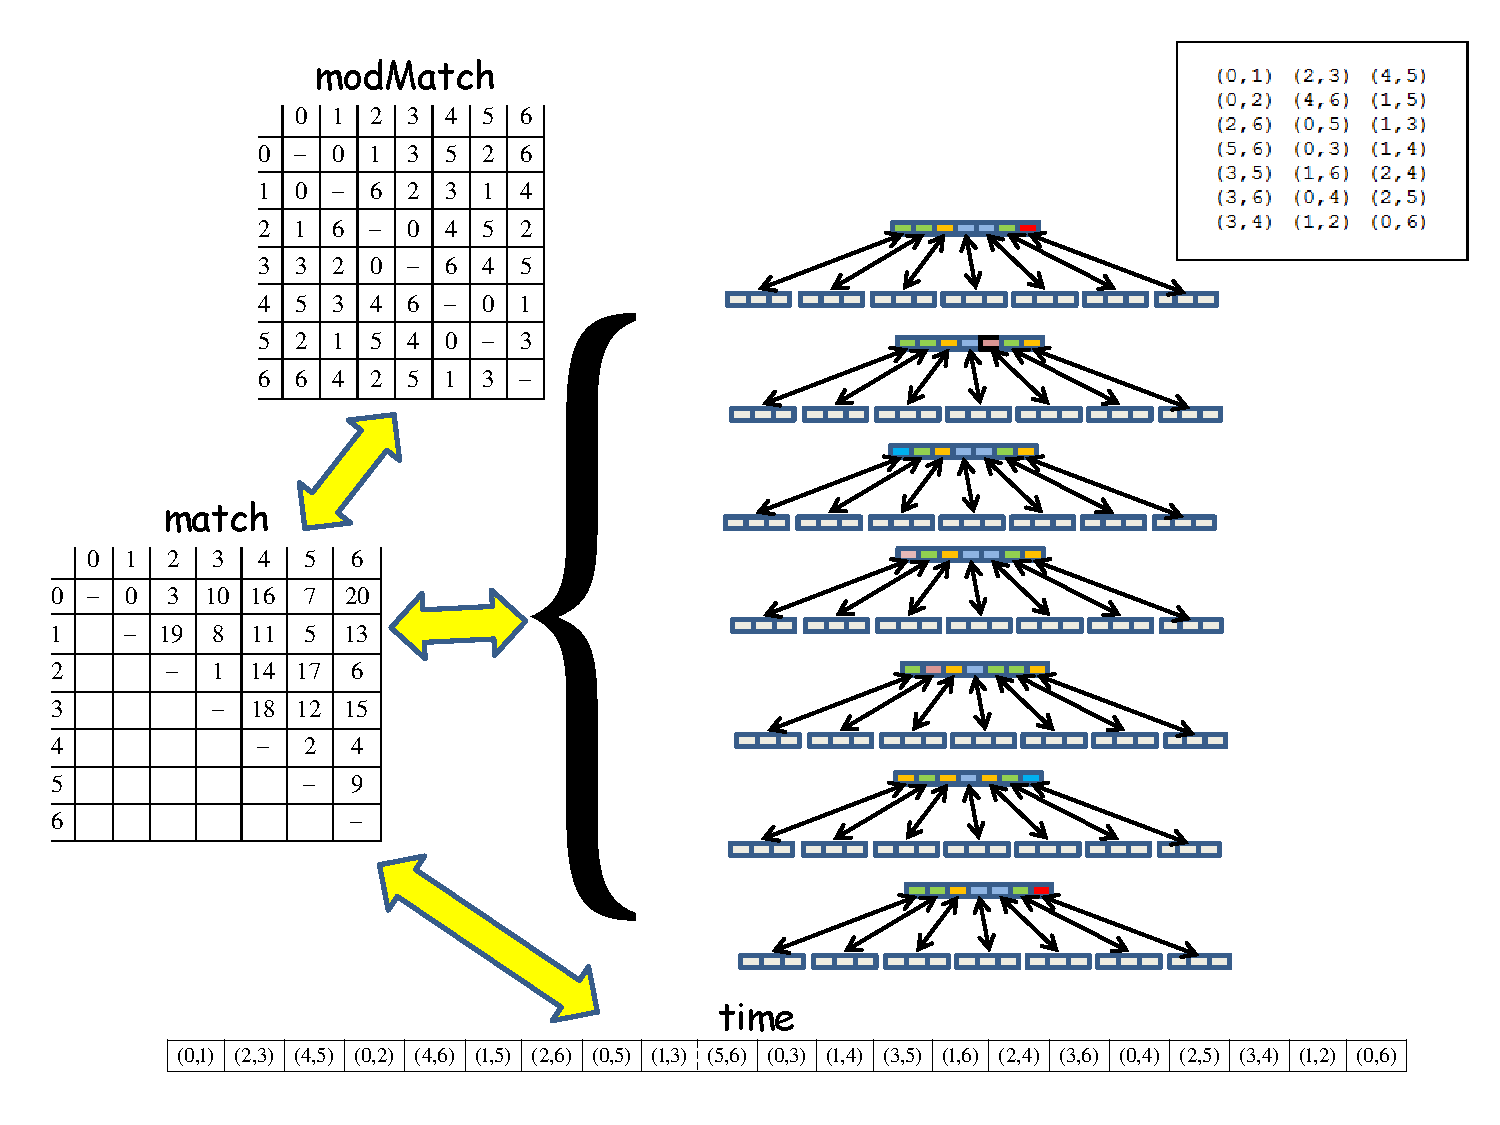
\includegraphics[height=10.2cm,width=13.2cm]{schedule.pdf}
\caption{A pictorial representation of the entire model of the schedule for 7
skippers and 6 boats. The schedule is reproduced top right. On the right we
have the 7 skippers, on top left the $\modMatch$ array, at the bottom
$\timeVar$ and middle left the $\match$ array. The yellow arrows signify
channeling between parts of the model.}
\label{schedChanges}
\end{figure}

\subsection{Stage 2: Minimising Imbalances}

Having produced a schedule that minimises boat changes, we then minimise
criteria 6, imbalance, by extending the model as in Figure~\ref{model:stage2}.
Assuming the first stage produced a schedule with $\beta$ boat changes we post
this as a hard constraint \eqref{C11} in stage 2. For each skipper $\sigma$ we
introduce a zero/one variable $position[{i,j}]$ \eqref{V9} which is 1 if and
only if skipper $\sigma$ is in a match in time $m \cdot j + i$, i.e.\ in the
$i^{th}$ match of the  $j^{th}$ flight \eqref{C12}. Imbalance \eqref{V10} is then computed
for each position, as the absolute amount of over or under
expected presence in a given position \eqref{C13}. Finally, we compute the
maximum imbalance over all positions for this skipper (\ref{V11}, \ref{C14}).

\begin{figure}[tb]
\setlength{\mathindent}{1em}
\setlength{\abovedisplayskip}{0pt}
\setlength{\belowdisplayskip}{0pt}
\setlength{\abovecaptionskip}{0pt}
\begin{framed}
\begin{align}
    \intertext{The objective value from stage 1 is used as a hard constraint:\smallskip}
    & \totalBoatChanges \leq \beta \tag{C11} \label{C11}
\end{align}
\end{framed}\begin{framed}
\begin{align}
    \intertext{A copy of these variables and constraints is created for each skipper $\sigma$:\smallskip}
    & \forall i \in \{ 0 \nldots m{-}1 \} : \forall j \in \{ 0 \nldots f{-}1 \} : \nonumber \\
    & \hspace*{1em} \position[{i,j}] \in \{0,1\} \tag{V9} \label{V9} \\
    & \hspace*{1em} \position[{i,j}] = 1 \Leftrightarrow \timeSlot[{m.j+i}] \geq 0 \tag{C12} \label{C12} \\
    & \forall i \in \{ 0 \nldots m{-}1 \} : \nonumber \\
    & \hspace*{1em} \imbalance[{i}] \in \mathbb{N} \label{V10} \tag{V10} \\
    & \hspace*{1em} \imbalance[{i}] = \abs*{\frac{n-1}{m} - \sum_{j=0}^{f-1} \position[{i,j}]} \label{C13} \tag{C13} \\
    & \maxImbalance \in \mathbb{N} \label{V11} \tag{V11} \\
    & \maxImbalance = \maximum(imbalance) \label{C14} \tag{C14}
\end{align}
\end{framed}\begin{framed}
\begin{align}
    \intertext{We minimise the maximum imbalance over all skippers:\smallskip}
    & \forall i \in \{ 0 \nldots n{-}1 \} : \imbalance[{i}] \equiv \sigma[{i}].\maxImbalance \label{V12} \tag{V12} \\
    & \maxImbalance \in \mathbb{N} \label{V13} \tag{V13} \\
    & \maxImbalance = \maximum(\imbalance) \label{C15} \tag{C15} \\
    & \minimise(\maxImbalance) \label{C16} \tag{C16}
\end{align}
\end{framed}
\caption{Additions to the constraint model in Figure~\ref{model:stage1} for
stage 2. The constant $\beta$ is the minimum number of boat changes found in
stage 1.}\label{model:stage2}
\end{figure}

We then capture the maximum imbalance over all skippers (\ref{V12}, \ref{V13}
and \ref{C15}) and minimise this \eqref{C16}. As before, the decision variables
are $\timeVar[{0}]$ to $\timeVar[{t-1}]$ and the same symmetry breaking is
imposed at top of search.

\subsection{Stage 3: Renaming Skippers}

Stage 3 then takes as input the schedule produced in stage 2 and renames
skippers in the last round of the last flight to be $(0,1)$, satisfying criteria
9. This is a simple linear process. The schedule produced for 7 skippers and 6
boats is shown in Table~\ref{tab2}.

\begin{SCtable}[1.8][tb]
    \setlength{\tabcolsep}{3pt}
    \begin{tabular}{cccc}
        \toprule
        Flight & \multicolumn{3}{c}{Matches} \\ \midrule
        0 & (0,6) & (2,3) & (4,5) \\
        1 & (0,2) & (4,1) & (6,5) \\
        2 & (2,1) & (0,5) & (6,3) \\
        3 & (5,1) & (0,3) & (6,4) \\
        4 & (3,5) & (6,1) & (2,4) \\
        5 & (3,1) & (0,4) & (2,5) \\
        6 & (3,4) & (6,2) & (0,1) \\ \bottomrule
    \end{tabular}
    \caption{A round-robin schedule with 7 skippers, 6 boats and 7 flights,
        which is the result of stages 1, 2, and 3. It has 6 boat changes
        and imbalance 1. An example of imbalance is skipper $\sigma[{0}]$
        with 2 matches in position 0 (first), 3 in position 1 and 1 (mid)
        in position 2 (last). Perfect balance would be 2 matches in each
    position, only achieved by skipper 2.}\label{tab2}
\end{SCtable}

\subsection{Stage 4: Orienting Matches}

The final stage, stage 4, orients skippers within matches, such that they are
either port (red) or starboard (green). This is done to satisfy criteria 2 and
3, 5 and 8. A sketch of the constraint model is given with a supporting
diagram, Figure~\ref{oriented}.  A sequence of zero/one constrained integer
variables, of length $n-1$, is produced for each skipper. These correspond to
the sequence of skippers they meet in matches. For example, taking the schedule
in Table~\ref{tab2}, skipper $\sigma[{2}]$ meets skippers in order:
3,0,1,4,5,6, and skipper $\sigma[{5}]$ in the order 4,6,0,1,3,2.  Therefore,
skipper $\sigma[{2}]$'s 4$^{th}$ variable must take a different value from
$\sigma[{5}]$ 5$^{th}$ variable. There are summation constraints on each
skipper to enforce criteria 2 and 3 (equal number of port and starboard
matches). Criteria 8 is enforced by posting constraints such that in a match
($\sigma[{i}],\sigma[{j}]$) where $\abs*{i - j} = 1$, the higher indexed skipper
(lower ranked) is on the port side. A DFA constraint is posted for criteria 5
(restricting sequences of port and starboard assignments).

In Figure~\ref{oriented}, port is red and starboard green. The sequence of
zero/one variables for each skipper is shown on the left. Bottom right is the
DFA, and top right is the final schedule produced from stages 1 to 4. The
schedule has 6 boat changes and a maximum imbalance of 1. Three days CPU time
was devoted to stages 1 and 2. Stages 3 and 4 completed in 15 milliseconds. The
schedule presented here is new, not appearing in the example schedules provided in \cite{isaf}.%ISAF World Sailing Umpire's Manual

\begin{figure}[tb]
\centering
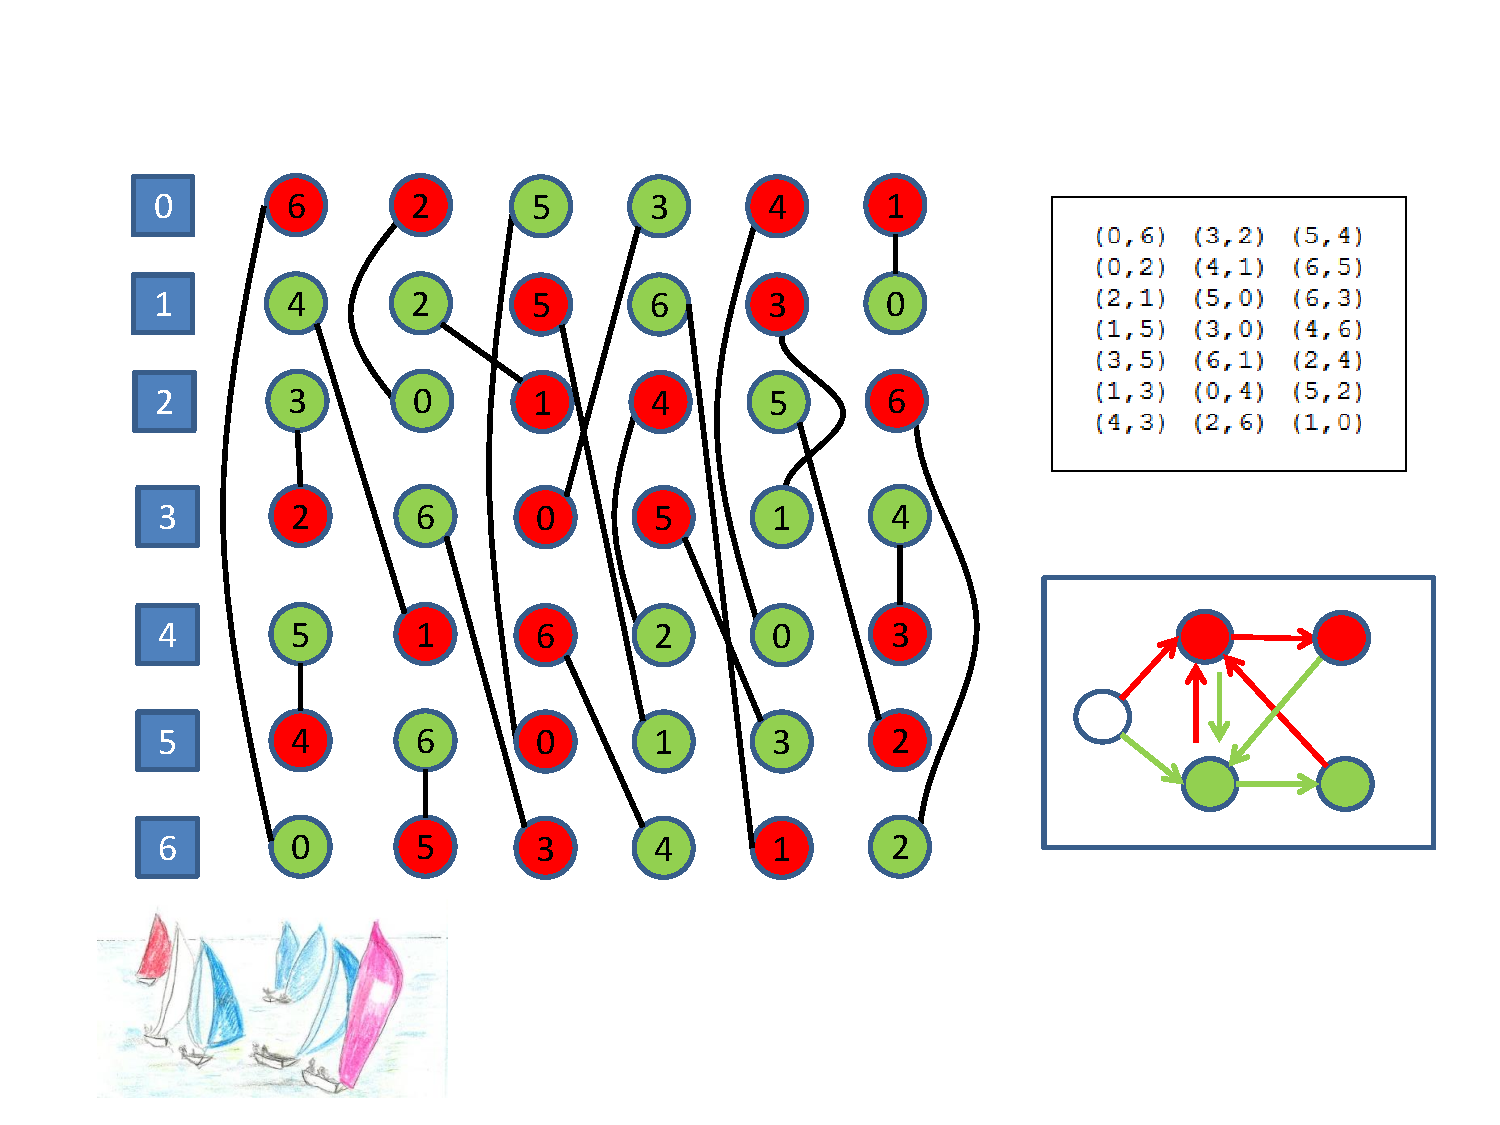
\includegraphics[height=10.2cm,width=13.2cm]{oriented.pdf}
\caption{A pictorial representation of the orientation process, stage 4. Top
right is the actual oriented schedule. Below that is the dfa to satisfy
criteria 5. On the left is the zero/one variables, a row representing a
skippers sequence of competitors. An edge between variables corresponds to a
matched pair, that must take different values. Bottom right is a sketch by third author.}
\label{oriented}
\end{figure}

\section{Sample Schedules}\label{sec:samples}

\begin{center}
\begin{figure}[h]
\begin{minipage}[t]{0.5\textwidth}
\hspace{0.6cm}
%\begin{scriptsize}
\begin{tabular}{cccc}
        \toprule
        Flight & \multicolumn{3}{c}{Matches} \\ \midrule
        0 & (5,2) & (4,3) & (1,6) \\ 
        1 & (4,2)  & (6,5) & (3,1) \\
        2 & (6,4) & (2,1) & (3,5) \\
        3 & (6,2) & (5,0) & (1,7) \\
        4 & (5,1) & (0,6) & (2,7) \\
        5 & (7,5) & (2,0) & (6,3) \\
        6 & (0,7) & (4,1) & (3,2) \\
       7 & (7,4)  & (0,3) &  \\
       8 & (4,0)  & (7,3) &  \\
       9 & (5,4)  & (7,6) & (1,0) \\ \bottomrule
          & & & \\
          & & & \\
    \end{tabular}
%\end{scriptsize}
\label{08-06a}
\end{minipage}
\hfill
\begin{minipage}[t]{0.5\textwidth}
\hspace{0.6cm}
%\begin{scriptsize}
\begin{tabular}{cccc}
        \toprule
        Flight & \multicolumn{3}{c}{Matches} \\ \midrule
        0 & (2,7) & (3,0) & (5,4) \\ 
        1 & (0,2)  & (4,3) & (7,5) \\
        2 & (0,4) & (7,6) & (5,3) \\
        3 & (4,6) & (5,0) & (3,1) \\
        4 & (6,5) & (3,2) & (1,4) \\
        5 & (6,3) & (4,7) & (2,1) \\
        6 & (7,3) & (1,6) & (4,2) \\
       7 & (7,1)  & (2,5) & (6,0) \\
       8 & (5,1)  & (0,7) & (6,2) \\
       9 & (1,0)  & & \\ \bottomrule
          & & & \\
          & & & \\
    \end{tabular}
%\end{scriptsize}
\label{08-06b}
\end{minipage}
\caption{Schedules for 8 skippers and 6 boats. On the left is the published ISAF schedule, and this is illegal. On the right is our schedule, respecting all ISAF criteria..}
\label{08-06}
\end{figure}
\end{center}


\begin{center}
\begin{figure}[h]
\begin{minipage}[t]{0.5\textwidth}
\hspace{0.6cm}
%\begin{scriptsize}
\begin{tabular}{cccc}
        \toprule
        Flight & \multicolumn{3}{c}{Matches} \\ \midrule
        0 & (0,7) & (3,2) & (5,4) \\ 
        1 & (0,2) & (7,4) & (5,3) \\
        2 & (4,0) & (7,3) & (2,5) \\
        3 & (3,0) & (2,4) & (6,5) \\
        4 & (4,3) & (5,1) & (8,6) \\
        5 & (3,1) & (6,2) & (4,8) \\
        6 & (6,3) & (1,4) & (8,2) \\
        7 & (4,6) & (2,7) & (1,8) \\
        8 & (7,6) & (0,8) & (2,1) \\
        9 & (8,7) & (5,0) & (6,1) \\
        10 & (8,5) & (1,7) & (0,6) \\
        11 & (7,5) & (3,8) & (1,0) \\ \bottomrule
    \end{tabular}
%\end{scriptsize}
\label{09-06}
\end{minipage}
%\hfill
\begin{minipage}[t]{0.5\textwidth}
\hspace{0.6cm}
%\begin{scriptsize}
\begin{tabular}{ccccc}
        \toprule
        Flight & \multicolumn{4}{c}{Matches} \\ \midrule
        0 & (0,6) & (3,2) & (5,4) & (1,7) \\
        1 & (2,0) & (6,3) & (4,1) & (8,7) \\
        2 & (6,4) & (0,5) & (7,2) & (3,8) \\
        3 & (4,7) & (1,8) & (0,3) & (5,2) \\
        4 & (3,1) & (7,5) & (8,0) & (2,6) \\
        5 & (3,7) & (4,8) & (2,1) & (6,5) \\
        6 & (8,2) & (1,6) & (5,3) & (0,4) \\
        7 & (5,1) & (7,0) & (6,8) & (4,3) \\
        8 & (8,5) & (2,4) & (7,6) & (1,0) \\ \bottomrule
        & & & & \\
        & & & & \\
        & & & & \\
    \end{tabular} 
%\end{scriptsize}
\label{09-08}
\end{minipage}
\caption{Two new schedules. On the left, 9 skippers and 6 boats and on the right 9 skippers and 8 boats.}
\label{09}
\end{figure}
\end{center}

\subsection{Discussion}
Having a constraint program for this problem has a number of unexpected advantages, in particular, we can now investigate the effect different criteria have on our ability to produce schedules and how relaxation of those affect optimisation criteria. That is, the constraint program can be used help design the next set of umpire's rules.

\section{Conclusion}\label{sec:conclusions}



\section*{Acknowledgments}
We would like to thank our parents, God, and all his angels.
%\coffee{2}

\bibliographystyle{plain}
\bibliography{bib}

\end{document}
